\chapter{Fundamentação Teórica}
Para dar ínicio ao nosso panorama geral revisaremos, neste capítulo, os conceitos básicos sobre som, o que é informação musical e como é feito o armazenamento no banco de dados, quais as representações e estruturas do áudio digital e por fim, a recuperação da informação musical.

\section{Conceitos Básicos sobre Som}
Nós ouvimos uma variedade de sons à todo momento, e vivemos toda a nossa vida rodeados por eles. Sons de portas abrindo e fechando, dos passos, do ruído dos motores dos automóveis, da chuva e da música. O som não é algo que podemos ver com nossos olhos \cite{miletto2004}. Então, o que é o som? 
Um som é gerado por algum objeto vibratório, em uma repetição periódica de deformações e restaurações \cite{muller2007}. Estas vibrações produzem mudanças de pressão do ar, resultando em regiões locais de ar que são mais densas e outras que são rarefeitas, ocorrendo sucessivamente uma depois da outra e expandindo-se. Estas são chamadas condensações e rarefações. O processo é similar ao que conhecemos quando jogamos uma pedra dentro d’água, a qual produz ondas circulares em sua superfície. Estas ondas de condensações e rarefações são propagadas para dentro do ouvido humano e irão vibrar o tímpano. As vibrações são captadas pelas terminações nervosas, de maneira que nós as escutamos como sons, ou então ser convertido em um sinal elétrico pelo microfone. Se os corpos que vibram são diferentes, também será diferente a classe de vibração que produzem, isto significa que escutamos distintas classes de sons.

Se essa pressão do ar varia de acordo com um padrão repetitivo dizemos que o som tem uma forma de onda periódica. Se não há um padrão perceptível no som este é chamado de ruído. E quando as variações na pressão do ar são representadas de forma gráfica, podem ser interpretadas como “formas de onda”. Na Figura \ref{fig:ondaSenoidal} a representação gráfica de um som mostra as mudanças na pressão do ar conforme a passagem do tempo. Lendo-se o gráfico da esquerda para a direita, quando a linha curva está próxima da parte inferior do gráfico, então a pressão do ar é mais baixa, e quando a curva está próxima do topo do gráfico, a pressão do ar aumentou \cite{miletto2004}.

\begin{figure}[!htb]
   \centering
   \caption{Representação gráfica, no domínio temporal, de uma forma de onda senoidal}\label{fig:ondaSenoidal} 
   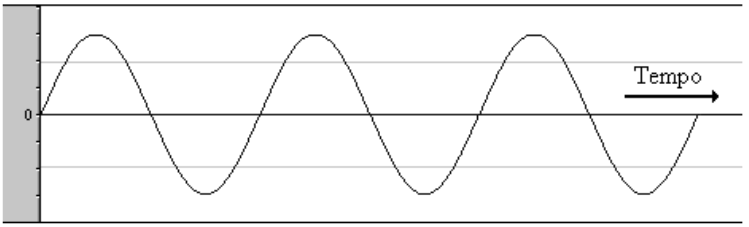
\includegraphics[scale=0.6]{figuras/ondaSenoidal.png}
   Fonte: \cite{miletto2004}.
\end{figure}

Os autores \citeonline{miletto2004} apresentam os quatro elementos básicos do som, que são:
\begin{enumerate}
\item Altura tonal: É a “altura” de um som, ou seja, se é alto ou baixo, agudo ou grave. A repetição de uma onda periódica é chamada de ciclo. O número de ciclos dentro do intervalo de um segundo é chamado freqüência, medida em hertz (Hz), que é então a recíproca do período. Quanto maior o valor em hertz, mais agudo é o som. Dobrando a freqüência de um som, este é elevado em uma oitava, então é possível dizer que a freqüência e a altura tonal estão relacionadas logaritmicamente.

\item Volume: A mudança no volume de um som pode ser vista como uma diferença na altura das ondas. A altura de uma onda chama-se “amplitude”. Quanto maior a amplitude, mais forte é o som. Portanto o volume de um som é determinado pela amplitude.

\item Timbre: É o que diferencia dois sons de mesma frequência. De um modo geral, formas de ondas arredondadas produzem um timbre mais suave enquanto que as formas de ondas ponteagudas dão um timbre mais penetrante e estridente.

Na Figura \ref{fig:ondaTimbre} são mostradas três formas de onda básicas, seus timbres característicos e os instrumentos que se assemelham a cada caso.

\begin{figure}[!htb]
   \centering
   \caption{Formas de onda simples e seus timbres}\label{fig:ondaTimbre} 
   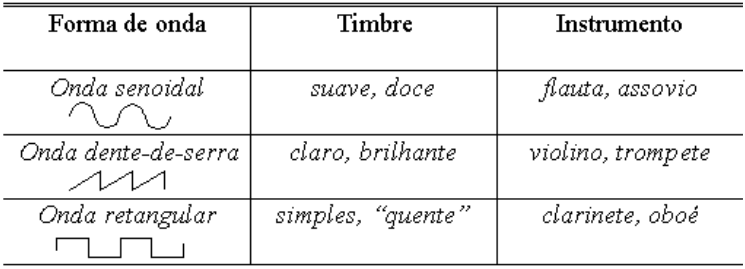
\includegraphics[scale=0.6]{figuras/ondaTimbre.png}
   Fonte: \cite{miletto2004}.
\end{figure}

\item Envolvente da Onda: É a variação da altura tonal, do volume e do timbre em um transcurso de tempo que vai desde o começo do som até um ponto do tempo onde ele desaparece completamente. Estas mudanças no tempo são o que determina o timbre característico de um objeto, além do seu espectro harmônico.
\end{enumerate}

Os sons com vibrações regulares - que são os harmônicos e a fundamental \footnote{Por definição, o primeiro harmônico corresponde à freqüência fundamental, o segundo harmônico ao primeiro harmônico e assim por diante \cite{muller2007}.} - são considerados sons musicais, enquanto os sons causados por vibrações irregulares - que não são harmônicos - cuja altura tonal não pode, portanto, ser medida, são chamados sons não-musicais. A maioria dos sons usados na música são, por pressuposto, sons musicais.

\section{Informação Musical}
Para \citeonline{miletto2004} o processo de representar numericamente o som é chamado de digitalização. Um som contendo freqüências limitadas pode então ser representado por uma seqüência de simbolos quantificados ou quantificáveis, ou seja, de números. Segundo \citeonline{setzer2001}, dado é uma sequencia de números, portanto, um texto, fotos, figuras, sons gravados e animação são dados, pois todos podem ser quantificados. Um dado é necessariamente uma entidade matemática e, desta forma, é puramente sintático. Isto significa que os dados podem ser totalmente descritos através de respresentações formais, estruturais e obviamente ser armazenados em um computador e processados por ele. O processamento de dados em um computador limita-se exclusivamente a manipulações estruturais dos mesmos, e é feito por meio de programas. Estes são sempre funções matemáticas, e portanto também são dados. Exemplos dessas manipulações nos casos de textos são a comparação com outros textos, etc.

Sendo o dado puramente sintático, ao incluir um “significado” implícito na palavra, usado para sua caracterização, é gerado a informação, que é necessariamente semântica.

O autor expõe que a informação é uma abstração informal (isto é, não pode ser formalizada através de uma teoria lógica ou matemática) que está na mente de alguém, representando algo significativo para essa pessoa. Utilizando-se da frase “Paris é uma cidade fascinante” é um exemplo de informação – desde que seja lida ou ouvida por alguém, desde que "Paris" signifique para essa pessoa a capital da França (supondo-se que o autor da frase queria referir-se a essa cidade) e "fascinante" tenha a qualidade usual e intuitiva associada com essa palavra.

A informação pode ser armazenada em um computador, ou melhor, a sua representação em forma de dados e não a informação propriamente dita. Essa representação pode ser transformada pela máquina, como na formatação de um texto (o que seria uma transformação sintática), mas não pode mudar o significado, já que ele depende de uma pessoa que possui a informação. Os dados são sempre incorporados por alguém como informação, porque os seres humanos buscam constantemente por significação e entendimento \citeonline{setzer2001}.

Á partir daí, a autora \citeonline{barros2012} expõe que um dado musical é resultado de um processo de significação social. Assim, a música é uma expressão humana construída socialmente e objetivada por meio de sua comunicação oral, registro sonoro ou representação gráfica.

Para \citeonline{almeida2007}, a obra musical é efêmera e abstrata, pois só se concretiza no momento de cada interpretação, na execução da música. \citeonline{berger&luckmann2014} afirmam que:

\begin{citacao}
A expressividade humana é capaz de objetivações, isto é, manifesta-se em produtos da atividade humana que estão ao dispor tanto dos produtores quanto dos outros homens, como elementos que são de um mundo comum.
\end{citacao}

Para \citeonline{angeles2010,pinheiro&loureito1995} a informação é o que se acrescenta a uma representação. Segundo o autor, recebemos informação se o que conhecemos é alterado. Informação é o que logicamente justifica alteração ou reforço de uma representação ou de um estado de coisas. As representações podem ser explícitas (como em um mapa, ou em uma proposição), ou podem estar implícitas no estado de atividade dirigida do receptor.

A informação musical apresenta determinadas especificidades de comportamento na sua produção, objetivação e uso, pois a manifestação da música apresenta-se carregada de características próprias. \citeonline{michels1992} explica que a música contém dois elementos: o material acústico e a ideia intelectual, sendo que tais elementos não se encontram justapostos, mas sim, se combinam para formar uma imagem unitária. Portanto, a compreensão completa da música está diretamente ligada com o reconhecimento do contexto histórico e social de sua origem, com a interpretação pessoal e individual do ouvinte, e com os aspectos sonoros que a constituem, dessa forma, a música tem diferente significações para cada indivíduo.

\citeonline{lima&santini2006} afirmam que:

\begin{citacao}
A música é um produto social e simbólico de grande importância nas diferentes formações culturais, principalmente se considerarmos a sua capacidade de criar vínculos afetivos e cognitivos entre as pessoas.
\end{citacao}

A compreensão da música como informação é ainda bastante recente. O estudo mais significativo e considerado, dentro da literatura especializada, como pioneiro na conceituação e estudo da música como fonte de informação é o de Alexander McLane. Em 1996 o autor publicou em um capítulo do ARIST \abreviatura{ARIST}{Annual Review of Information Science and Technology} o artigo intitulado \textit{Music as Information} onde formaliza a música como informação.

\section{Armazenamento da Informação Musical}

Até o surgimento dos inventos tecnológicos, a música era um meio de comunicação exclusivamente presencial. Apesar das formas de registros, a exemplo das partituras, possibilitarem a execução de uma obra em diferentes momentos e lugares, a reprodução do que ali estava representando nunca seria a mesma. Com o decorrer do tempo as técnicas e invenções aplicadas ao processo de gravação do som foram surgindo e se aperfeiçoando, resultando em aparelhos reprodutores e suportes cada vez mais versáteis e manipuláveis \cite{daquino2012}. Especialmente após o desenvolvimento das coleções em rede na web, com formatos de arquivos compactados e custos decrescentes de armazenamento de arquivos na forma digital, a música se tornou um objeto de consumo universal e extremamente acessível \cite{gomes2015}.

Os dispositivos de armazenamento musical são divididos em dois grandes grupos: analógicos e digitais \cite{andrade&crispim2008}. Os analógicos são antecessores dos digitais e foram o meio tecnológico dominante em boa parte do século XX \cite{paulozuben2004}. O primeiro invento significativo foi o fonógrafo, patenteado por Thomas Edison em 1877. Dez anos mais tarde, em 1887, surgiu o gramofone, tendo uma capacidade maior de armazenamento e reprodução das músicas \cite{marchi2005}. 

Dentre as invenções mais importantes para o armazenamento e a reprodução sonora analógica está o disco de vinil, lançado em 1948, comumente conhecido como LP\abreviatura{LP}{long-play}. Era um disco com rotação por minuto mais demorada, o que permitia aumentar a capacidade de armazenamento da informação na superficie do vinil. Em seguida, entre as décadas de 60 e 70, com a evolução dos cartuchos 8-track (pioneiros em armazenar dados musicais em fitas magnéticas), o lançamento da fita cassete ou compact cassette \cite{marchi2005}, era basicamente, dois carretéis, a fita magnética e todo o mecanismo de movimento da fita, alojados em uma caixa plástica \cite{andrade&crispim2008}.

No armazenamento analógico, as formas de onda dos sinais elétricos emitidos do aparelho eram registradas similarmente, isto é, de maneira análoga, pelas partículas magnéticas encontradas na fita. No momento da reprodução, os sinais magnéticos impressos na fita são interpretados analogamente como diferenças de voltagem, isto é, sinais elétricos. Como o nível do sinal elétrico era muito baixo, utilizava-se um amplificador para que a variação de voltagem estivesse suficiente para mover os cones dos alto-falantes. Dizemos que esse processo é uma gravação analógica, pois a forma de onda do sinal gravado é análoga à forma de onda do sinal original captado \cite{paulozuben2004}.

Porém a paritr da década de 80, com a intensificação do uso de \textit{hardwares} e \textit{softwares}, surge um dos primeiros meios de
armazenamento digital: o CD \abreviatura{CD}{Compact-Disc}. E acabou por se tornar um dos meios de armazenamento de dados musicais mais populares das décadas seguintes. Além de quebrar paradigmas na época, o CD foi inspiração para o desenvolvimento de outros meios de armazenamento como os DVDs\abreviatura{DVD}{Digital Versatile Disc} e os discos de Blu-ray \cite{marchi2005}.

Entretanto surgiu a necessidade de disponibilizar informações no dispositivo de armazenamento. Na era analógica esses recursos estavam associados à capa e/ou contracapa. Todavia, com a mudança do paradigma para digital, necessitou-se que essas informações pudessem ser disponibilizadas digitalmente, porém o CD de áudio não inclui em sua estrutura, por exemplo, o nome do disco ou o nome de suas faixas. Sendo assim, surgiram as bases de dados de CDs que visam prover informações dos mesmos quando esses são utilizados por sistemas de mídia modernos \cite{andrade&crispim2008}.

Com o surgimento dos arquivos digitais de áudio, as músicas se desvincularam do suporte físico (CD) e passaram a ser vistas isoladamente e esses tipos de arquivos requerem um espaço consideravel para seu armazenamento (chegando a ocupar dezenas de megabytes em disco), o que propiciou o surgimento de um formato mais compacto: O MP3 \abreviatura{MP3}{Moving Picture Experts Group-1 Layer 3}. 

O grande desenvolvimento tecnológico das redes de compartilhamento de arquivos contribuiram para uma maior aceitação de formato de áudio MP3 \cite{andrade&crispim2008}, por ser facilmente transportado em qualquer bolso ou mochila e pela sua longa vida útil, além do aumento gradativo de armazenamento com o passar dos anos \cite{marchi2005}.

Sua invenção, propiciou a a popularização de eletrônicos com portas USB e o surgimento de cartões de memória microSD, prometendo maior capacidade, durabilidade e clareza sonora \cite{marchi2005}.

Com a internet, a música ultrapassa os limites físicos da mídia, mergulhando no universo digital, a música passa a circular livremente pela rede mundial de computadores através do \textit{streaming} que tomou forma no final da década de 80 e começou a se desenvolver na década de 90, com a evolução dos SGBDs \abreviatura{SGBD}{Sistemas de Gerenciamento de Banco de Dados} e o surgimento dos BDOOs \abreviatura{BDOO}{Banco de Dados Orientado a Objetos} \cite{junior&segundo2008}, que possibilitou o armazenamento de multimidias e a primeira rádio online surgiu em 1994. Assim como a popularização de aplicativos móveis, conhecido normalmente por app, que oferecem mais de 30 milhões de música a seus usuários, por exemplo, "Spotify"\footnote{https://www.spotify.com/br/} e "Deezer"\footnote{https://www.deezer.com/br/}.

A evolução dos arquivos musicais não foi acompanhada de tentativas de inserção de informações elementares da música a esses arquivos. Há pouco tempo não existia um padrão para a representação dos metadados associados a esses arquivos \cite{andrade&crispim2008}. E a recuperação dessa informação só será bem sucedida se esses documentos multimídias puderem ser representados de acordo com as suas peculiaridades \cite{gomes2015}.

\section{Representação e Estruturas da Informação Musical}

O som é a variação da pressão do ar. Sendo assim, a forma de produzir um determinado som depende da maneira como a pressão do ar varia \cite{miletto2004}. A digitalização das formas de onda consiste em duas etapas: \textbf{amostragem} e \textbf{quantização}. Na primeira etapa, a forma de onda é lida ou amostrada em intervalos de tempo uniformes. Então, na segunda etapa, o valor da forma de onda em cada ponto amostrado é restrito ou quantificado para um conjunto discreto de valores. É uma transformação com perdas, no sentido de que se perde informação neste processo. Veja a Figura \ref{fig:ondaAnalog} para uma ilustração.

\begin{figure}[!htb]
   \centering
   \caption{Forma de onda analógica (curva preta) e representação digitalizada (os valores digitalizados são indicados pelas caixas cinzentas). Neste exemplo, a forma de onda é amostrada em 24 pontos e a quantização dos valores emprega um esquema de codificação de 4 bits (16 valores possíveis)}\label{fig:ondaAnalog} 
   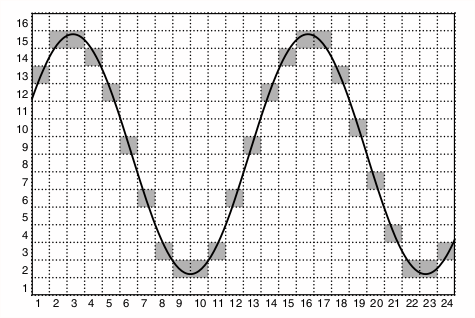
\includegraphics[scale=0.9]{figuras/ondaAnalog.png}
   Fonte: \cite{muller2007}.
\end{figure}

Armazenar dados de áudio em formato analógico discretizado consome muito espaço \cite{juliana2004}, e como solução foi adotada a codificação MIDI \abreviatura{MIDI}{Musical Instrument Digital Interface}. Essa codificação é uma representação da informação musical, e é usado atualmente como o formato de intercâmbio de música digital simbólico mais comum para possibilitar a transferência de informações entre instrumentos musicais e computadores \cite{muller2007}. E o tamanho desses arquivos, tende a ser bem reduzido, já que a codificação de eventos musicais pode ser bem compacta.

Embora isso seja satisfatório em algumas situações, arquivos MIDI (extensão .mid ou .smf) basicamente codificam apenas instruções referentes a notas e durações e não a informação sonora propriamente dita \cite{fernando&kon1998}. Ou seja, seu código são instruções para um sintetizador, correspondentes a eventos musicais como soar uma nota, silenciar uma nota, mudar o andamento ou o tom da música, etc. O sintetizador, por sua vez, interpreta este código e o executa, podendo usar vários timbres de instrumentos simultaneamente \cite{miletto2004}, e por isso, o resultado sonoro é totalmente dependente da qualidade e das possibilidades oferecidas por esse aparelho \cite{fernando&kon1998}.

Com o mesmo objetivo, os formatos Wave, da Microsoft (extensão .wav) e AIFF, da Apple (extensão .aiff ou .aif) são do tipo áudio digitalizado sem compressão. Baseiam-se na codificação PCM \abreviatura{PCM}{Pulse Code Modulation}, onde a própria onda sonora é representada como uma sucessão de números correspondentes às amplitudes do sinal medidas a uma freqüência constante. Ou seja, armazenam dados de um processo de digitalização simples. A diferença para com o formato MIDI, é que esse tipo de codificação origina um grande volume de dados e exige muito espaço para armazenamento e sua única vantagem é a reprodução fiel do áudio, se o arquivo for gravado com qualidade de CD \cite{miletto2004}.

Outro recurso é a compressão de dados que é feita através de programas ou hardware específicos que compactam os arquivos de áudio, reduzindo o seu tamanho, antes de serem enviados. Ao chegar ao seu destino, esses arquivos são descompactados e, em seguida, tocados. Entretanto, compressão, nesse contexto, é sinônimo de perda de qualidade: quanto maior a compressão, maior, também, a quantidade de informação que se perde \cite{fernando&kon1998}. Apesar disso, certos padrões de compressão já permitem a transmissão de arquivos de áudio de boa qualidade em tempo real, o que resulta na existência de uma quantidade equivalente de formatos de arquivo para a compressão do som digitalizado \cite{miletto2004}.

Segundo \citeonline{miletto2004}, os formatos de arquivo mais utilizados para a compressão de som são:

\begin{itemize}
   \item Sun Audio, da Sun (extensão .au);
   \item Real Audio, da RealNetworks (extensão .ra);
   \item MPEG Layer 3 (extensão .mp3);
   \item Windows Media Audio, da Microsoft (extensão .wma).
 \end{itemize}

\section{Recuperação da Informação Musical}

A área de pesquisa denominada \textit{Music Information Retrieval}(MIR \abreviatura{MIR}{Music Information Retrieval}) ou Recuperação da Informação Musical (RIM \abreviatura{RIM}{Recuperação da Informação Musical}), tradução literal incorporada pela corrente da área no Brasil.

De acordo com \citeonline{futrelle&downie2002} a Recuperação da Informação Musical é:

\begin{citacao}
[...] uma agenda de pesquisa que, de forma geral, pretende desenvolver formas de gestão de coleções de obras musicais para preservação, busca, acesso e outros usos.
\end{citacao}

A agenda de pesquisas sobre a RIM intensificou sua produção recentemente com a explosão do interesse em coleções em rede que contenham obras musicais na forma digital, possibilitadas pelo desenvolvimento das citadas técnicas de compressão de áudio. Os pesquisadores de RIM observam que a motivação maior para essa área de pesquisa é o grande volume de música digital disponível na Internet que quanto mais cresce menos possibilita sua recuperação eficiente visto que estão apenas disponíveis aos montes, mas sem o tratamento adequado \cite{gomes2015}.

A área de RIM conta com profissionais das mais diversas áreas inclusas na questão do tratamento e recuperação da informação musical como apresentado na tabela a seguir, traduzida por \citeonline[p.11]{santini&souza2007}

\begin{figure}[!htb]
   \centering
   \caption{Comunidades de RIM}\label{fig:comunidadeRim} 
   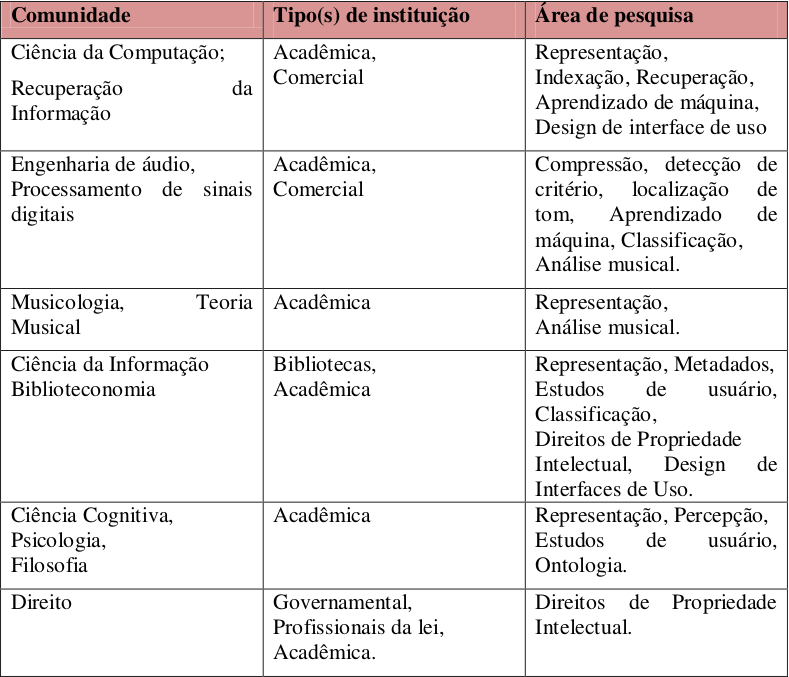
\includegraphics[scale=0.6]{figuras/comunidadeRim.png}
   Fonte: \cite{futrelle&downie2002}.
\end{figure}

A origem de RIM não apresenta uma ação interdisciplinar, o que prejudica todo o seu processo de comunicação científica. Como pontua \citeonline[p.11]{santini&souza2007}:

\begin{citacao}
(...) não há uma sociedade (inter)disciplinar de RIM; um periódico ou livro-texto fundador onde pessoas interessadas podem adquirir as bases teóricas e práticas de RIM. Com exceção de alguns pequenos encontros interdisciplinares, muitos pesquisadores estão apresentando seus resultados para membros das suas próprias disciplinas. A literatura de RIM é difícil de ser localizada, lida e estudada, o que dificulta construir e sustentar uma área de pesquisa respeitável, próspera.
\end{citacao}

A escassa produção científica a respeito do tema e as características impostas pelas músicas acarretam em certas dificuldades para sua representação.

Como elucidado no final do item 2.1 deste capítulo, o ponto de partida para os estudos sobre a música como fonte de informação e tratamento, representação e recuperação foi dado em 1996 por Alexander McLane. Neste mesmo período já era possível identificar o desenvolvimento de tecnologias de compressão de arquivos digitais de música para transmissão na Internet e a popularização da Internet no mundo \cite{santini&souza2007}.

Em seu estudo McLane direciona sua discussão para os grandes problemas relacionados à representação de documentos de música e à recuperação destes documentos. McLane analisa aspectos significantes da música – sua notação e seu som – e propõe algumas ideias para sistemas de recuperação de música, e formaliza a música como informação segundo três visões: visão subjetiva, visão objetiva e visão interpretativa. Segundo o autor, as necessidades dos vários tipos de análises musicais são tão diversas que é preferível considerar três “visões” sobre a representação da obra musical.

Em resumo adaptado, \citeonline{santini&souza2007} apresenta as principais características das visões estabelecidas por \citeonline{mclane1996}.

\begin{itemize}
    \item A visão \textbf{subjetiva} da informação musical se faz por meio do uso do esquema de notação para representação da informação musical. A subjetividade se dá porque a escolha de elementos de notação geralmente representa uma obra em “contexto-dependente” sendo assim a decisão da notação pode incluir ou excluir aspectos particulares da obra.
    \item A visão \textbf{objetiva} está vinculada a audição e ao momento da execução musical. Um som gravado pode ser identificado como visão objetiva da obra musical. A sonoridade se caracteriza como objetiva por não se configurar como uma representação, mas como a obra em sua essência. O som musical uma vez gravado torna-se fixo e não está mais sujeito a variações editoriais e de performance. Segundo McLane esta visão pode ser considerada a mais completa representação da música, ao passo em que inclui as facetas: tom, tempo, harmonia, editorial e timbre.
    \item A visão \textbf{interpretativa} é realizada através da análise de alguns aspectos da obra, engloba informações que não são diretamente dependentes do documento. Entram nessa categoria classificações e esquemas analíticos que elucidam características como o gênero musical e avaliações críticas.
\end{itemize}

De acordo com \citeonline[p.11]{cruz2014}:

\begin{citacao}
Dentre as visões propostas por McLane (1996), a interpretativa possui uma característica interessante porque permite a independência formal do documento musical em relação ao suporte que o contém, assim como foi possível na informação textual.
\end{citacao}

Segundo \citeonline[p.5]{mclane1996,santini&souza2007}, a representação da informação musical pode abranger as três visões apresentadas dependendo das necessidades de informação da comunidade usuária. De acordo com tradução das autoras, a conclusão de McLane seria a de que:

\begin{citacao}
Ambas as escolhas sobre a visão da representação da música e o grau de complementação da representação de uma obra depende da necessidade de informação do usuário. A recuperação de informação é um processo interativo que depende do conhecimento do usuário e do nível de complexidade da informação desejada. No caso da necessidade da simples identificação de uma obra musical, onde a informação bibliográfica não é unicamente suficiente, pode-se limitar a uma visão subjetiva envolvendo um subconjunto relativamente pequeno de elementos notados de uma obra, frequentemente o tom inicial de uma frase melódica. A representação tonal pode ser de forma tal que provavelmente o usuário espera e está apto para formular a indagação usando a mesma terminologia, ou pelo menos uma que é traduzível na forma de representação.
\end{citacao}

Sendo assim, percebe-se que a recuperação da informação da música depende tanto da complexidade e da forma como a informação é representada como do nível de conhecimento prévio do usuário. Para \citeonline[p.5]{santini&souza2007}: “Quanto menor o conhecimento do usuário, maior a necessidade de diferentes formas de representação. Cada visão da representação da música, demonstrada por McLane, não é suficiente isoladamente para identificar uma obra.”.

Outro autor presente nos estudos relacionados à representação e recuperação de informação musical e um dos representantes da área de RIM é o professor J. Stephen Downie da Universidade de Illinois, nos Estados Unidos. Downie escreveu, em 2003, outro artigo tido como marco no estudo da informação musical, intitulado Music Information Retrieval também em um capítulo do ARIST. No trabalho em questão, \citeonline{downie2003} examina a multidisciplinaridade da área de RIM, identifica e explica alguns problemas relacionados a questão da representação e recuperação da informação musical. Para isso \citeonline{downie2003} resume a questão em quatro grandes desafios a serem enfrentados pelos pesquisadores da área.

De acordo com \citeonline[p.5]{downie2003,santini&souza2007} os quatro desafios seriam:

\begin{citacao}
    \begin{enumerate}
        \item Considerar permanentemente as diferentes formas de representação da música, o que caracteriza o \textbf{desafio multirepresentacional}. O copyright faz parte deste desafio.
        \item Cada época histórica e cada formação cultural criam modos próprios e singulares de se expressar através da música. A música transcende as fronteiras culturais e temporais. A ampla variedade de expressões musicais coloca em evidência o \textbf{desafio multicultural}.
        \item Compreender e responder às diferentes formas de interação individual com a música e com os sistemas de RIM constitui o \textbf{desafio multiexperimental}.
        \item Maximizar os benefícios de ter uma comunidade multidisciplinar de pesquisadores, enquanto minimiza a desvantagem inerente, representa o \textbf{desafio multidisciplinar}.
    \end{enumerate}
\end{citacao}

O desafio multirepresentacional é dividido em sete facetas a serem consideradas na descrição da música e que representam a estrutura musical \cite{downie2003}. São elas: tonal, temporal, harmônica, de timbre, editorial, textual e faceta bibliográfica. Sendo as quatro primeiras relativas a aspectos sonoros da música com formas gráficas de representação em figuras rítmicas ou notações musicais, enquanto que as três últimas são representadas na forma gráfica e dizem respeito às informações de produção, intérprete, compositor, copyright, data de produção e outras \cite{barros2012}.

Apesar de completas, a interação dessas facetas resulta em um complexo tratamento da informação musical, visto que cada faceta citada possui por si só uma complexidade inerente e sofre um tipo de representação enquanto produto. As autoras \citeonline[p.8]{santini&souza2007} resumem a problemática multirepresentacional da seguinte forma:

\begin{citacao}
    A complexa interação entre as facetas da música - tempo, harmonia, timbre, freqüência, editoria, texto e bibliografia – evidencia um dos principais problemas de RIM: o desafio multirepresentacional. A escolha da representação da música – se baseada em símbolos, áudio ou ambos – adiciona-se a diversas questões: como, por exemplo, cada escolha determina a tecnologia, a organização, a recuperação e a interface entre requisitos e capacidades dos sistemas.
\end{citacao}

Sendo assim, apesar de possuir as facetas estabelecidas pelo autor, a estrutura da música incorpora elementos extras que nos permitem defini-la como um objeto informacional mais complexo. Além das facetas definidas por \citeonline[p.283]{downie2003,cruz2014}, a estrutura musical:

\begin{citacao}
    [...] incorpora elementos adicionais que permitem defini-la como um objeto informacional musical mais amplo, dotado de conteúdo – atributos internos e metadados descritivos – e, de contexto – associações com outros objetos musicais e não musicais, e com situações ou eventos em que este objeto musical está inserido.
\end{citacao}

O segundo desafio (multicultural) nasce da condição inerente à música de ser uma objetivação de algo extremamente subjetivo: a expressão humana. Sendo assim, sofre a interferência de uma grande variedade de fatores, da cultura vigente no momento da produção musical e da localização geográfica desta produção.

O desafio multiexperimental diz respeito à percepção da música como experiência individual ou coletiva capaz de causar diferentes reações em diferentes momentos e situações, de cada mente e humor individual. Neste caso ouvir uma música gravada funciona como “ajudar a memória” que traz a tona experiências prazerosas ou dolorosas relacionadas a uma música em especial \cite{downie2003,santini&souza2007}. As variações de pessoa para pessoa na forma de apropriação, apreciação e nos tipos de experiências emocionais que a música evoca demonstram de maneira pragmática o desafio multiexperimental.

O quarto e último desafio estabelecido por \citeonline{downie2003} é o desafio multidisciplinar. Como citado anteriormente, a diversidade intelectual da comunidade de pesquisadores de RIM é, ao mesmo tempo, uma vantagem e uma adversidade. A heterogeneidade das visões de mundo das disciplinas apresenta um problema particular. Cada disciplina traz suas crenças, práticas, questões de pesquisa e paradigmas de avaliação \cite{downie2003}. De acordo com \citeonline{futrelle&downie2002}, não há uma aceitação comum dos objetivos, técnicas e resultados obtidos nas pesquisas referentes à informação musical.

Percebe-se por tanto, que se por um lado, a ação multidisciplinar dos pesquisadores envolvidos com o tema possibilita o surgimento de diversos avanços tecnológicos e que a cada dia são divulgadas novas soluções para o tratamento de conteúdos musicais, com algoritmos mais sofisticados, novas formas de indexação de músicas, novos tipos de interfaces de áudio e novas formas de representação musical, em contrapartida, é notável a dificuldade de comunicação entre esses resultados. Nota-se ainda a dificuldade de identificação desses conteúdos musicais, porque a música é complexa e possui um leque de propriedades que possibilitam abordagens, às vezes, contraditórias \cite{cruz2014}.

A análise documental da informação musical para sua representação apresenta complexidades, pois exige diferentes técnicas de extração de informações para distintas formas de apresentação \cite{downie2003}.

\subsection{Técnicas e Métodos para Recuperação da Informação}

Um dado multimídia geralmente é representado por um conjunto de características extraídas do conteúdo do dado. Isto porque dados multimídia são basicamente arranjos multidimensionais de valores derivados de vários sensores, que é uma representação limitada para definir a semântica do dado. Neste sentido, dados complexos raramente são comparados diretamente. Em vez disso, o conteúdo do dado (ou uma faceta do conteúdo) é analisado por meio de algoritmos especializados de análise, extraindo um conjunto de características, que descrevem numericamente o dado. Desta forma, um dado multimídia pode ser representado como um ponto no espaço de características, de acordo com o valor extraído para cada uma das características. Representando dados complexos em um espaço de características, torna-se possível estabelecer relações de similaridade entre os dados \cite{kaster2012}.

Dadas as características de um sinal de áudio, pode-se definir métricas de similaridade para comparar músicas.

\subsubsection{Dynamic Time Warping}

O \textit{Dynamic Time Warping} (DTW\abreviatura{DTW}{Dynamic Time Warping}) (Keogh et al., 2005) é uma técnica que permite definir uma métrica entre séries temporais, por exemplo, características de áudio. Dadas duas séries \({Q}\) e \({C}\) de tamanhos \({n}\) e \({m}\), respectivamente, cria-se uma matriz \({D}\), \({n\times m}\), onde o elemento \({d_{i,j}}\) é a distância entre o elemento \({q_{i}}\) e \({c_{j}}\).

A partir da matriz \({D}\), o algoritmo procura por um caminho mínimo \({W}\), onde \({w_{k} = (i,j)_{k}}\), que respeite as seguintes condições:

\begin{itemize}
    \item Comece em \({(1,1)}\) e termine em \({(n,m)}\);
    \item Percorra apenas índices adjacentes;
    \item Percorra espaçamentos iguais no tempo.
\end{itemize}

O caminho mínimo é encontrado por meio de um algoritmo de programação dinâmica de complexidade \({O(nm)}\) (Keogh et al., 2005). A métria de dissimilaridade DTW é dada por:

\begin{equation}
    DTW(Q,C) = \sqrt{\sum_{k=1}^{K} D[w_{k}]}
\end{equation}

, em que \({K}\) é o tamanho do caminho e \({D[w_{k}]}\) é o valor da entrada \({(i,j)_{k}}\) na matriz \({D}\). A Figura \ref{fig:dtw} ilustra a execução do algoritmo DTW.

\begin{figure}[!htb]
   \centering
   \caption{Execução do algoritmo de DTW. (A) Séries C e Q. (B) Matriz de distâncias. (C) Alinhamento das duas séries com o caminho mínimo.}\label{fig:dtw} 
   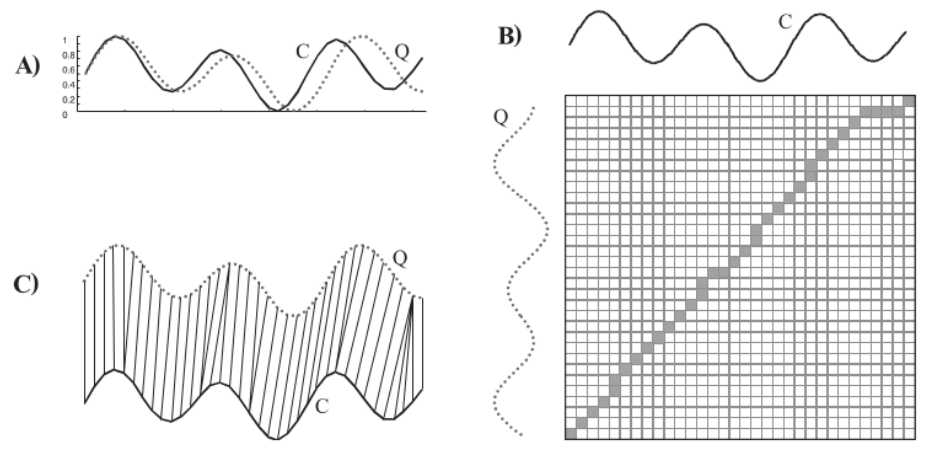
\includegraphics[scale=0.47]{figuras/dtw.png}
   Fonte: \cite{ono2015}.
\end{figure}

\subsubsection{Cross Recurrence Plot}

O trabalho de Serrà et al. (2009) propõe o uso de \textit{Cross Recurrence Plots} (CRP\abreviatura{CRP}{Cross Recurrence Plots}) como métrica de similaridade entre músicas. Antes de definir CRP, é necessário introduzir o conceito de \textit{Recurrence Plot} (RP\abreviatura{RP}{Recurrence Plot}). RP é uma ferramenta utilizada para visualizar recorrências com uma série temporal, ou seja, regiões onde a órbita da série passa perto de um estado previamente visitado. Mais especificamente, RP é uma matriz quadrada preenchida com zeros e uns, que indicam se há ou não recorrência, ou seja, se o estado no tempo \({i}\) é similar ao estado do tempo \({j}\) (Eckmann et al., 1995; Alligood et al., 2000). A diagonal principal de um RP é, portanto, composta por uns. CRPs sao construídos da mesma maneira que RPs, mas cada eixo corresponde a uma série temporal diferente e a matriz resultante não é quadrada.

Primeiramente, o algoritmo extrai a característica HPCP (Gomez, 2006) de duas músicas, resultando em séries temporais de \({H = 12}\) variáveis. Dados os vetores HPCP da música \textbf{\({x}\)} e da música \textbf{\({y}\)}, calcula-se a transposição de \textbf{\({y}\)} de modo que ela fique na mesma tonalidade de \textbf{\({x}\)}. A transposição ocorre rotacionando-se o vetor HPCP de \textbf{\({y}\)} em \({k}\) posições, por meio da técnica \textit{Optimal Transposition Index}, proposta em (Serra et al., 2008).

A seguir, calcula-se o \textit{embedding} das duas músicas em um espaço de fase, isto é, um espaço onde as recorrências do sinal podem ser obtidas. Considere que  HPCP \textbf{\({x}\)} tem \({N_{x}^{*}}\) janelas. O \textit{embedding} de \textbf{\({x}\)} é dado por \({x' = \big\{x_{i}\big\}}\), para \({i = 1, ..., N_{x}, N_{x} = N_{x}^{*} - (m - 1)*\tau}\), em que \({x_{i}}\) é calculado com:

\begin{gather}
    x_{i} = (x_{1,i},x_{1,i+\tau}, ..., x_{1,i+(m-1)\tau},\\
             x_{2,i},x_{2,i+\tau}, ..., x_{2,i+(m-1)\tau},\\
                                                   ...\\
             x_{H,i},x_{H,i+\tau}, ..., x_{H,i+(m-1)\tau})
\end{gather}

Os autores estimaram os valores ótimos de \({m}\) e \({\tau}\) para o reconhecimento de músicas \textit{cover}, por meio da divisão de uma base de dados em conjunto de treinamento e teste: